\setlength{\parskip}{1em}

\chapter{Introduction}

\section{Radiative Transfer in Astrophysics}

Electromagnetic radiation, or light, is how we perceive and understand the universe. It also acts as a critical driver of the evolution of astrophysical systems and is an efficient transporter of energy over large distances, allowing systems to cool and collapse and to heat their surroundings. Thus, radiation is a key regulator for the evolution of astrophysical systems, limiting processes like star and galaxy formation. It is the dominant feedback contributor (as a fraction of energy output) of stellar systems as well as driving ionization and chemistry. Despite this, it is often neglected or treated very approximately due to its difficulty and computational cost. In this thesis we explore the challenges of including radiative transfer in simulations of astrophysical systems.

As an example, star formation requires cool gas whose thermal pressure can be overcome by gravity, allowing the gas cloud to collapse. Radiative heating and gas stripping \citep{gasStripping} will thus limit the quantity of gas available for star formation.

The required mass for a gas cloud to overcome thermal pressure and begin collapsing into a star, known as the Jeans Mass ($M_J$), is related to the temperature of the gas such that
\begin{equation}
    M_J \propto T^\frac{3}{2}.
\end{equation}
This implies that the effects of heating and cooling by radiation are of great importance to the dynamics of star-forming regions, with an increase of temperature of a factor of ten leading to a greater than thirty-fold increase in the mass required to collapse. A common approximation is to allow radiation to escape instantly. This is quite wrong given that these clouds block a large portion of the visible, ionizing and thermal radiation.

Additionally, radiation pressure can cause the expulsion of gas from star forming regions. As stars tend to form in tight clusters, the first stars to form will affecet the properties of those that follow as their high luminosity removes available gas from the region. We know that star formation is very inefficient compared to the free-fall time. It is commonly assumed that early feedback must play a key role in preventing too much star formation. Without including radiation this interaction can only be modelled through the addition of numerical estimators.

Figure \ref{fig:lumvsage} shows the luminosity per solar mass as a function of time from a simulated star cluster. It can be seen that the total luminosity, and thus energy, of the system is dominated by radiation. The far UV (FUV) and extreme UV (EUV) bands also play a vital role in heating and ionization effects. As solar wind is driven by the optically thick metal lines in the UV spectrum, the only remaining energy contribution to luminosity is supernovae, whose energy input is exceeded by many orders of magnitude across almost the entire lifetime of the star and occurs late, almost certainly after star formation has slowed in the original cloud.

\begin{figure}[H]
    \centering
    \includegraphics[width=\textwidth]{"./plots/CH1/uvsn"}
    \caption{Luminosity per solar mass against time for a simulated stellar population made in Starburst99 and using a Chabrier initial mass function \citep{starburst}. Plot recreated by Jasper Grond. \citep{grond}}
    \label{fig:lumvsage}
\end{figure}

\subsection{The Basics of Radiative Transfer}

For an optically thin system with a single source, the flux $\bm{F}$ received by a sink object is given by,
\begin{equation}
\label{eqn:flux}
\bm{F} = \frac{L}{4\pi |\bm{r}|^3}\bm{r},
\end{equation}
where $L$ is the luminosity of the source and $\bm{r}$ is the vector between source and sink. As with gravity, the total flux received by an object from multiple sources is simply the sum of all fluxes, i.e.,
\begin{equation}
\bm{F} = \sum_{i}{\frac{L_i}{4\pi |\bm{r}_i|^3}}\bm{r}_i,
\end{equation}
where $\bm{r}_i$ and $L_i$ are the values of $\bm{r}$ and $L$ for the $i$th source in the system. In the case of an absorbing medium the flux is reduced exponentially by the optical depth $\tau$. This gives,
\begin{equation}
\bm{F} = \sum_{i}{\frac{L_i}{4\pi |\bm{r}_i|^3}\bm{r}_i e^{-\tau_i}},
\label{eqn:fluxThick}
\end{equation}
where $\tau_i$ is defined as the distance integral $ds$ of the intervening material's absorption coefficient $\alpha$ along the line defined by $a_i$ and $b_i$. $\alpha$ is a function of the materials properties such as composition, density and temperature,
\begin{equation}
    \tau_i = \int_{a_i}^{b_i}{\alpha(s) ds}.
    \label{eqn:tau}
\end{equation}
Additionally, the luminosity and absorption coefficient of objects depend substantially on the wavelength being studied, thus giving the full equation for the flux received by a sink from all sources,
\begin{equation}
\bm{F} = \int_{0}^{\infty}{\bigg( \sum_{i}{\frac{L_{i,\nu}}{4\pi |\bm{r}_i|^3}\bm{r}_i e^{-\int_{a_i}^{b_i}{\alpha_{\nu}(s) ds}}}\bigg) d\nu}.
\end{equation}
This ignores scattering which greatly increases the complexity of the system and is outside of the scope of this thesis. For further details see \citet{R&L}.

\section{Radiative Transfer Methods}

\subsection{Computational Complexity of Radiative Transfer}
While radiative transfer is vital to the understanding of our universe, simulating it comes with a high computational cost. This led to many codes choosing to omit radiative transfer or to include simple only estimates such as uniform flux fields. Nevertheless, there have been several attempts to produce accurate models of radiative transfer in astrophysical simulations that are discussed below. We discuss our own method (TREVR) in Chapter 2.

The most rudimentary method for ray tracing, equivalent to the ``brute force" $\mathcal{O}(N^2)$ method seen in gravity where N is the number of mass elements in the system, is where a ray is traced between every single sink and source pair. For the optically thin case, i.e. one with no absorption, this has a cost of $\mathcal{O}(N_{sink} N_{source})$. 

Unlike with gravity, where the interaction between two particles is unaffected by the intervening matter, radiation can be blocked through absorption or scattering of the ray's component photons. To perform ray tracing, all particles between the sink and the source must be sampled and the optical depth calculated from their properties. Assuming a uniform distribution of sinks this could require sampling of up to $n_{sink}^{\frac{1}{3}}$ particles (assuming sinks also act as absorbers), giving a maximum cost of $\mathcal{O}(N_{sink}^{\frac{4}{3}} N_{source})$, or $\mathcal{O}(N^{\frac{7}{3}})$ if the sinks and sources are well mixed and of similar number. As with gravity, there are a multitude of methods to reduce this to a more manageable level.

\subsection{Moment Methods}
Moment methods use simplified versions of the moments of the radiative transfer equations that allow for them to be easily computed through the use of partial differential equations. 

One method is Flux Limited Diffusion (FLD), so named due to the flux being limited to a value no greater than the radiation energy density times the maximum speed that the radiation is transferred \citep{FLD}. In this method, angular moments of the radiative transfer equations are computed in a frame rotating with the fluid and assume local thermodynamic equilibrium \citep{M&M1984}. 

The radiation energy density, $\bm{E}$, is given by,
\begin{equation}
    \bm{E}(\bm{r}, t) = \frac{1}{c}\int_{4\pi} d\bm{\Omega}\, I(\bm{r}, \bm{\Omega}, t),
\end{equation}
where I is the specific intensity of the radiation, a function of position ,$\bm{r}$, solid angle, $\bm{\Omega}$, and time, $t$, and c is the vacuum light speed. By integrating over all solid angles we get,
\begin{equation}
    \frac{\delta \bm{E}}{\delta t} + \bm{\nabla\cdot F} = c\alpha (B - E),
\end{equation}
where B is the radiation energy density for a black body emitter, $\alpha$ is the absorption coefficient and $\bm{F}$ is the radiative flux given by,
\begin{equation}
    \bm{F}(\bm{r}, t) = \int_{4\pi} d\bm{\Omega}\,\bm{\Omega}I(\bm{r}, \bm{\Omega}, t).
\end{equation}
By assuming that the intensity of the system is a slowly varying function of space and time (i.e. the diffusion limit), we can derive a function for the flux in terms of the gradient of the energy density (for a full derivation see \citet{FLD}),
\begin{equation}
    \bm{F} = -\frac{c}{\alpha}D_f\nabla E.
\end{equation}

Likewise, this can be done for the pressure tensor, giving an equation in terms of $\textbf{E}$. This can then be used with the energy density of each point on the mesh to give an estimate for both the flux and radiation pressure. Unfortunately, this has the issue of the diffusion of radiation around objects. This destroys sharp shadows and thus is a poor fit for simulations where the effects of shadowing are important.

These methods allow one to use a mesh, simplifying the data structures required but can require more complex methods when updating the fluxes between mesh cells such as the M1 method used by RAMSES-RT \citep{ramses} where flux, $\bm{F}$, is used as a dynamic variable alongside the energy density, $\bm{E}$.

\subsection{Monte-Carlo Methods}

Monte-Carlo methods use random elements to control the dynamics of a simulation. Originally developed as the ETRAN code in the 1960s \citep{ETRAN}, it is applied to radiation through the tracking of packets of photons from the source of emission until they either leave the simulation volume, or all energy is absorbed by intervening matter. Some Monte Carlo simulations such as MOCCASIN \citep{MC1} track the total energy of the packets. Each packet would have an equal energy and thus, for longer wavelengths a higher photon count. This avoids needing large number of packets for these regions of the spectra \citep{MC2}. Alternatively, it is possible to track the photon count, allowing for the total energy of the packet to change for packets of different wavelengths. Through this method, it is possible to terminate packets whose wavelengths are below values of interest (such as 13.6eV if studying hydrogen ionization), thus saving memory and computing time. By using this method, \citep{MC6} were able to run a grid of $128^3$ cells with only 1GB of RAM.

When a photon packet encounters an absorber in the Monte Carlo approach it is treated probabilistically and either fully absorbed or transmitted. Thus it must decide whether absorption occurs. This can be done by using a normalized cumulative probability function of the optical depth,
\begin{equation}
    P(l) = \frac{\int_{0}^{\tau_{\nu_p}(l)} e^{-\tau_{\nu_p}} d\tau_{\nu_p}}{\int_{0}^{\infty} e^{-\tau_{\nu_p}} d\tau_{\nu_p}} = 1 - e^{-\tau_{\nu_p}(l)},
\end{equation}
where $\tau_{\nu_p}(l)$ is the optical depth for a packet of wavelength $\nu_p$ and path length $l$ \citep{MC1}. This gives a value between 0 and 1 that can be compared to a random number of the same range which then gives the position that the energy packet is absorbed.

Alternatively, the inverse method can be used where a random number $U_R$ also in the interval [0, 1] is selected and then the optical depth calculated, as shown in \ref{Eqn:inverseMC}. From this optical depth, the path length can then be calculated \citep{MC4},
\begin{equation}
    \label{Eqn:inverseMC}
    \tau_{\nu_P}(l) = -\ln(1 - U_R).
\end{equation}

Once a large number of packets have been traced through the simulation box, the properties of each absorbing particle or grid cell can be calculated from the accumulated properties of all packets that interacted with them. 

The greatest issue with Monte-Carlo methods is the severe computational cost. High resolution estimates of properties such as mean intensity require large numbers of photon packets to be traced. Due to the number of photons in each direction obeying Poisson statistics, the error in each direction is given by,
\begin{equation}
    \sigma_E \approx \frac{E}{\sqrt{N}},
\end{equation}
where E is the total energy and N is the packet count, thus showing that the error scales poorly with packet count \citep{MC5}.

\subsection{Ray Tracing}

Ray tracing is a radiative transfer method where photon packets are ``traced" through the simulation along a finite number of linear rays, interacting with intervening matter and the propagation is generally assumed to be so fast that the speed of light is effectively infinite. This is correct for very slowly evolving systems (those close to a steady state) or where a physical process such as ionization is the rate limiting step rather than the speed of light. While many Monte-Carlo methods such as those seen in \citep{MCRT} utilize ray tracing methods to propagate radiation, pure ray tracing methods lack the stochastic absorption or iteration seen in combined methods outside of scattering where iteration is often necessary to find equilibrium \citep{DART}.

A key issue with ray tracing is that the resolution of absorbers depends on the distance between the absorber and the source. Assuming an equal number of rays in each direction there is a high density of rays near the source which falls off with an inverse-square profile as the distance increases, as shown in figure \ref{rayfig}. This means that to get a high sample rate for distant absorbers, a larger number of rays must be cast. This causes the closer absorbers to interact with a larger number of rays and incurs a greater computational cost.

\begin{figure} [H]
    \centering
    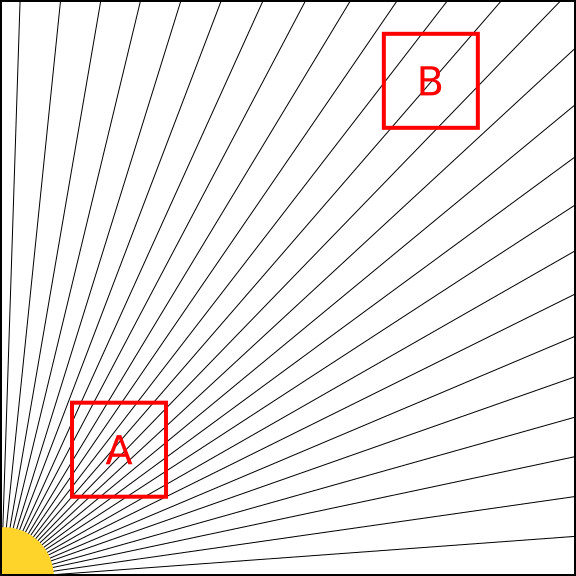
\includegraphics[width=\textwidth]{plots/CH2/rayDensityComparison.png}
    \caption{Ray density of a single source. Both regions A and B have the same area but region A intersects a far greater number of rays than region B.}
    \label{rayfig}
\end{figure}

One method used to mitigate this issue is to dynamically merge and split rays as they propagate so as to match the resolution of either the cells or the SPH particles such as is discussed in \citep{MORAYish} and implemented in MORAY \citep{moray}. This method utilizes a HEALPix sphere (see section \ref{sec:healpix}) of rays with equal solid angle where the number of rays at the source is fixed. As the rays interact with cells, they are checked against a refinement criterion where the number of rays intersecting the cell is logged. If there are too few rays, each ray is split into 4, with each child ray's direction set to give equal solid angles for all children. Likewise, if there are too many rays, the rays are collapsed into a single ray whose direction is the averaged direction of all child rays. This causes the number of rays sampling each cell to remain within set bounds and allows for a far more even sampling rate across the entire simulation box. Monte-Carlo methods that use rays for radiation propagation can also use this technique. 

While ray tracing is an excellent fit when looking to study the entire geometry of the system, it may not be the best method when looking to model scattering or if the distance individual rays travel is low. In this case, it may be preferred to use a simpler method such as FLD or to combine FLD with ray tracing algorithms.     

\section{Parallel codes and motivation}

Due to the high computational cost of radiative transfer, we need a large amount of computational power to run simulations with a high enough resolution to be realistic. This requires the use of High Performance Computing (HPC), where we utilize either very high clock rate single core processors or a combination of many processors into a multi-core system.

\subsection{The Limitations of Single Core Processors}

The two key methods to reduce computational cost without sacrificing resolution are the use of a processor with a greater clock speed or the use of multiple processors in unison. Single core processor speeds are closely linked to the size of their transistors which have historically reduced by a factor of two approximately every 18 months (a trend commonly known as Moore's Law). 

As the transistor gates decrease in size, electrons are more likely to quantum tunnel through the transistor gate, rendering them ineffective as transistors must reliably block the flow of electrons when closed. This places a limit on how small classical transistors can be manufactured before quantum effects begin to dominate.

The long running trend of the power usage remaining steady, regardless of the number of transistors, was also broken in the early 2000s due to the higher rate of thermal leakage in smaller transistors. The power draw is now approximately proportional to the cube of the transistor count, thus drastically increasing as we further reduce the transistor size. 

These issues, combined with the limitations on the amount of memory accessible to single core processors, makes it a challenge to scale simulations to high resolutions. This has led to the current standard of using multi-core systems.

\subsection{High Performance Computing}

The solution to the issue of high power usage in single cores has been to move from increasing the number of transistors to creating multiple cores on one chip. 2 cores running at half speed draw approximately a quarter of the power of a single core running at full speed while providing the same rate of computation. In principle, this not only reduces the cost of powering the system but also also reduces the amount of waste heat created. As cooling is often one of the larger expenses for data centres, this has a substantial impact on running costs.

Unfortunately, creating software that can run on multiple cores comes with many challenges. To discuss these, we will look at two types of parallel data management systems; shared data, where all cores have access to all data, and distributed data, where the data is distributed among multiple cores and each core only has access to its ``local" data.

With shared data, all cores are able to easily access any data they need and there is no need to synchronize each core but problems arise when multiple cores need to modify the same variable. As an example, say you have a function that adds to a shared integer. If a core attempts to access the integer while another is modifying its value, the core will fail to take into account the other core's contribution and thus return an incorrect value. Such issues are referred to as race conditions and require careful planning to avoid. This method also suffers from scaling limitations as the cores need to be within close physical proximity to the data storage medium to reduce latency.

Distributed data, on the other hand, stores a portion of the data set locally and in general is designed to only act directly on these data (e.g. with a gravity simulation, each core would calculate the gravitational force acting on each of their particles). This removes the possibility of a race condition for reads and writes as only one core is writing to any piece of data. It is still possible to create other similar issues but that is up to the programmer. Unfortunately, distributing data in such a way requires a far larger overhead as non-local data must be collected from other cores via message passing. The amount of data being stored on each core must be balanced with the rate and latency of data requests to ensure that the run time isn't dominated by message passing. The key benefit of distributed data is that the data is no longer bound to one storage device, allowing for the computation to be performed in multiple locations, possibly even multiple countries. This allows for access to far more memory and thus enables big problems to be tackled. For systems where latency isn't an issue, this can be used to take advantage of the vast computational power of consumer electronics, distributing computation to millions of personal computers and allowing for far greater data analysis than any one data centre could ever provide. An example of this is the BOINC software developed by the University of California \citep{boinc} where people can join programs to analyze massive data sets for such things as climate science and astrophysics.

To most effectively take advantage of parallel processing, the software must distribute the work among the cores in a way that minimizes the amount of time where multiple cores are idling while waiting for others to complete their tasks. This is known as Load Balancing. Typically this is also tied to the distribution of data (and thus limited by memory constraints per node).

\section{Summary of Thesis}

In Chapter 2, we look at the TREVR method for radiative transfer along with other existing methods for reverse ray tracing. We briefly discuss GASOLINE, the code base where TREVR was first implemented and how tree codes can be utilized to decrease computational cost.

Chapter 3 covers the implementation and methodology of the radiative transfer code in ChaNGa, discussing the key components of the Charm++ system and giving a detailed summary of the algorithms used.

Chapter 4 is focused on testing and analysis of the code, looking at the scaling of the method and finding appropriate values for the refinement parameters. 

Chapter 5 identifies the issue of complex sources as one not satisfactorily resolved in the original implementation of TREVR. We look at methods for resolving this without causing substantial increases to the algorithms computational cost.